\documentclass[11pt]{article}
\usepackage[a4paper,margin=28mm]{geometry}
\usepackage{pdfpages}
\usepackage[hidelinks]{hyperref}
\pdfinclusioncopyfonts=1
\begin{document}
\pagestyle{empty}
\thispagestyle{empty}
\begin{center}
{\LARGE Coset residues and chamber orbits}\\[12pt]
{\large Complete source disposition for L029}\\[8pt]
Human Compression project
\end{center}
\bigskip
This volume concerns D.~Leemans and P.~Tranchida,
\emph{On residual connectedness in chiral geometries},
Algebraic Combinatorics \textbf{4} (2021), 491--499,
\href{https://doi.org/10.5802/alco.162}{doi:10.5802/alco.162}.
The final journal edition is the fixed target.

The principal theorem is false for the full automorphism group in its
stated definition of chirality. The accepted five-page counterexample
is reproduced unchanged. The new synthesis supplies complete proofs of
the valid coset and residue arguments, and records the smaller auxiliary
corrections without conflating them with the principal error.

\bigskip
\begin{tabular}{p{.74\linewidth}r}
\textbf{Contents}&\textbf{PDF pages}\\[5pt]
Coset residues and chamber orbits&2--8\\[5pt]
A chiral coset geometry with disconnected residues&9--13\\[5pt]
Panels in the coset construction for a $C^+$-group&14--16\\[5pt]
Chirality without firmness&17--18
\end{tabular}
\bigskip

Each manuscript retains its own pagination and bibliography. The three
appended manuscripts retain their accepted bytes and proofs. All exact
TeX inputs are supplied. A plain incidence diagram in the synthesis
shows the seven-object auxiliary example.

General firmness in rank at least four, without an added action
hypothesis, remains unproved. Its status is distinct from that of the
source's false unrestricted statement. The finite checks certify their
specific examples; the general proofs are written arguments. No new
open-question solution, Lean result or compression factor is claimed.

The accompanying ledgers identify source ideas, retained project proofs,
corrections, and borrowed background.
The public principal-refutation record remains the record of the
counterexample; this volume completes its surviving source obligations.
\clearpage
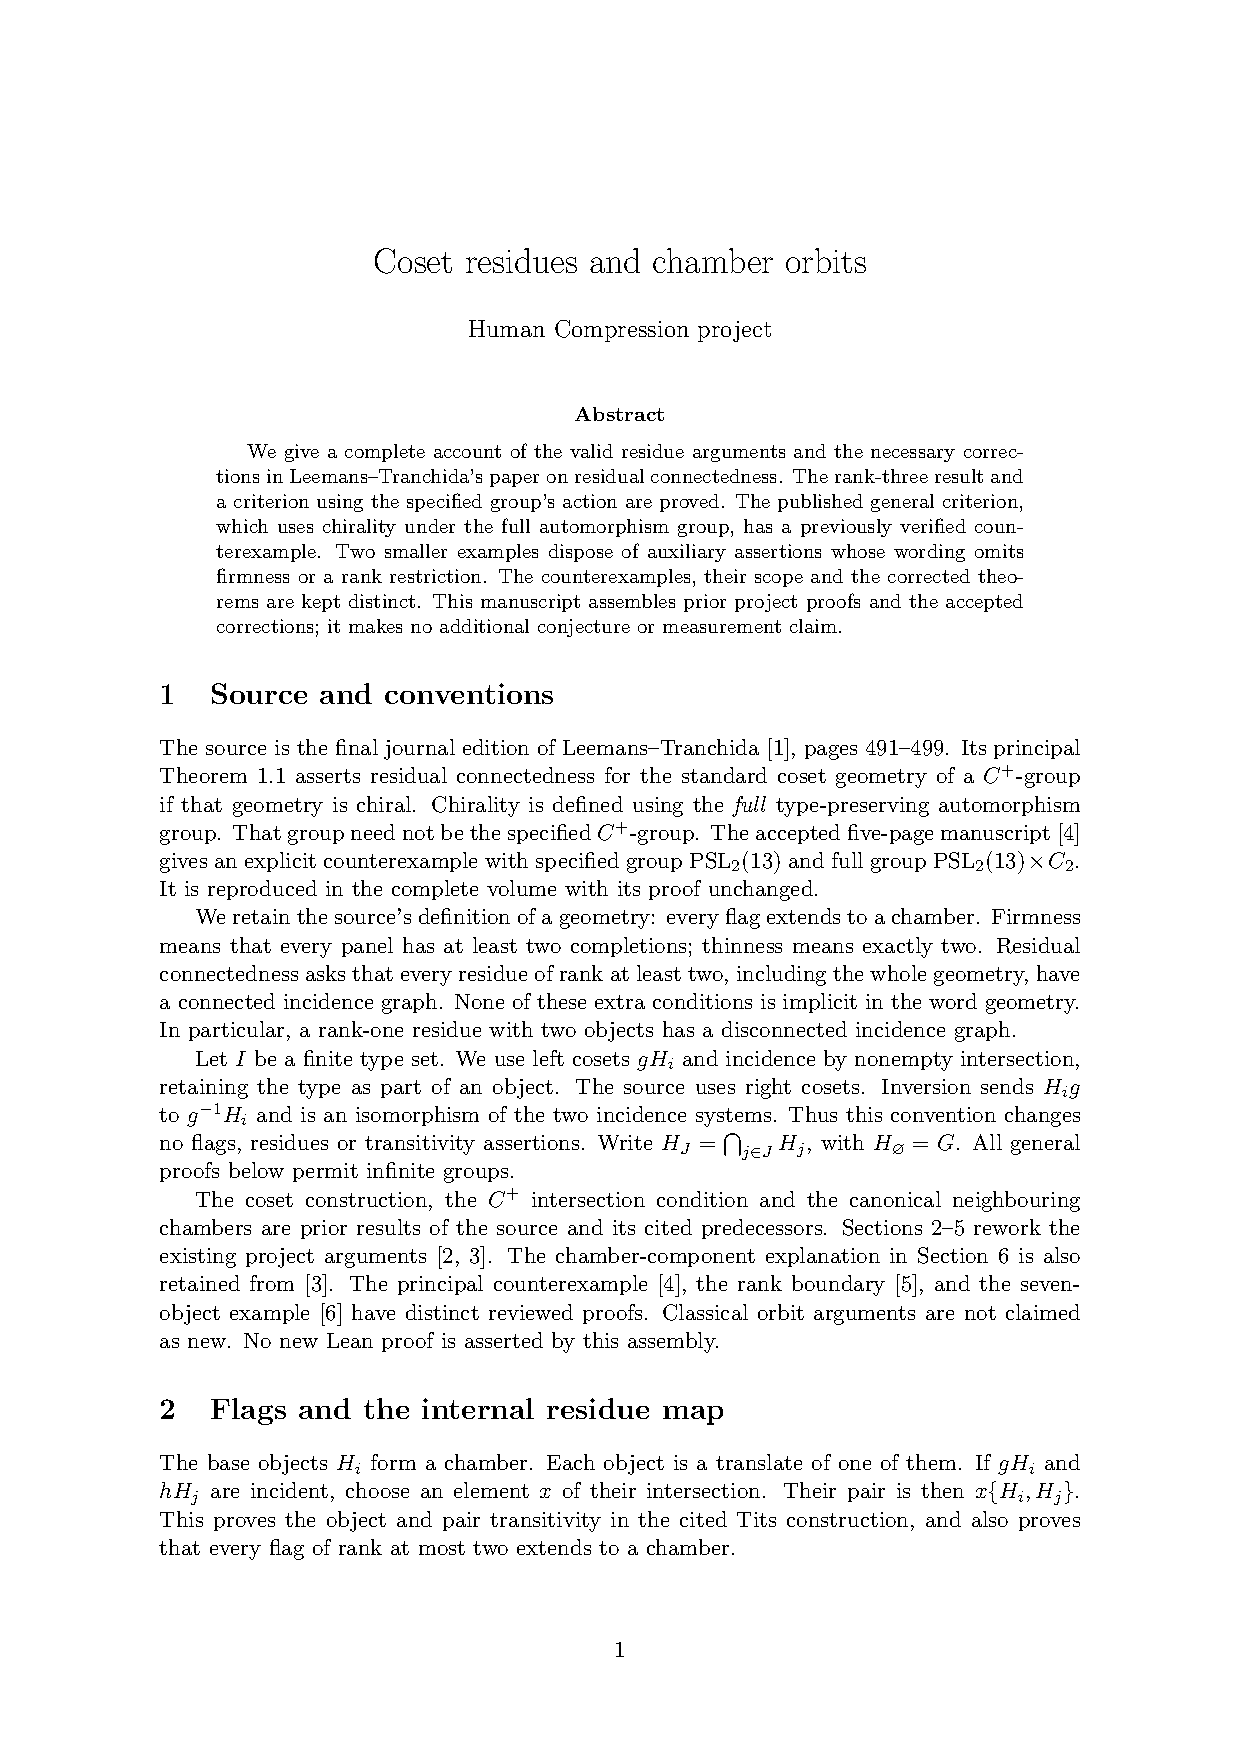
\includepdf[pages=-,pagecommand={},addtotoc={1,section,1,{Coset residues and chamber orbits},theory}]{residues.pdf}
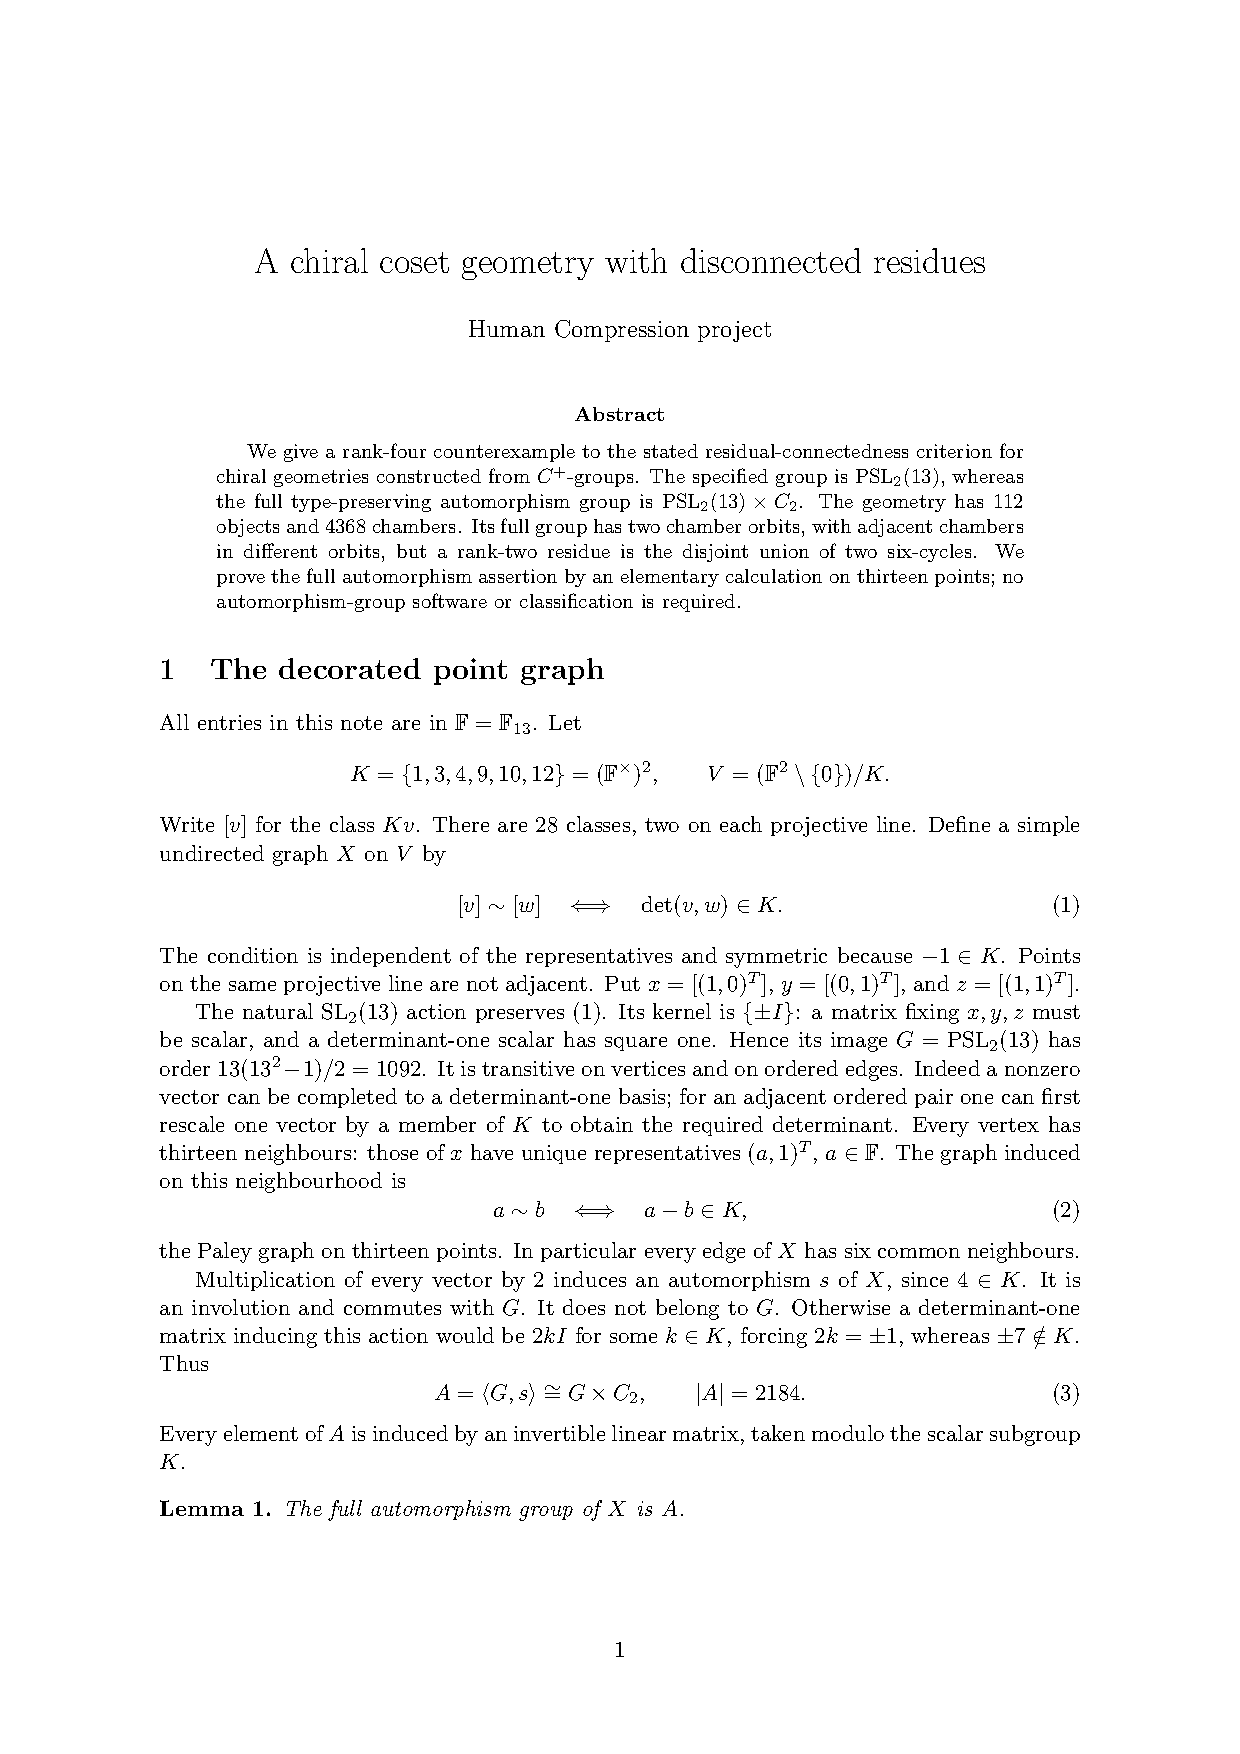
\includepdf[pages=-,pagecommand={},addtotoc={1,section,1,{A chiral coset geometry with disconnected residues},principal}]{proofs/principal.pdf}
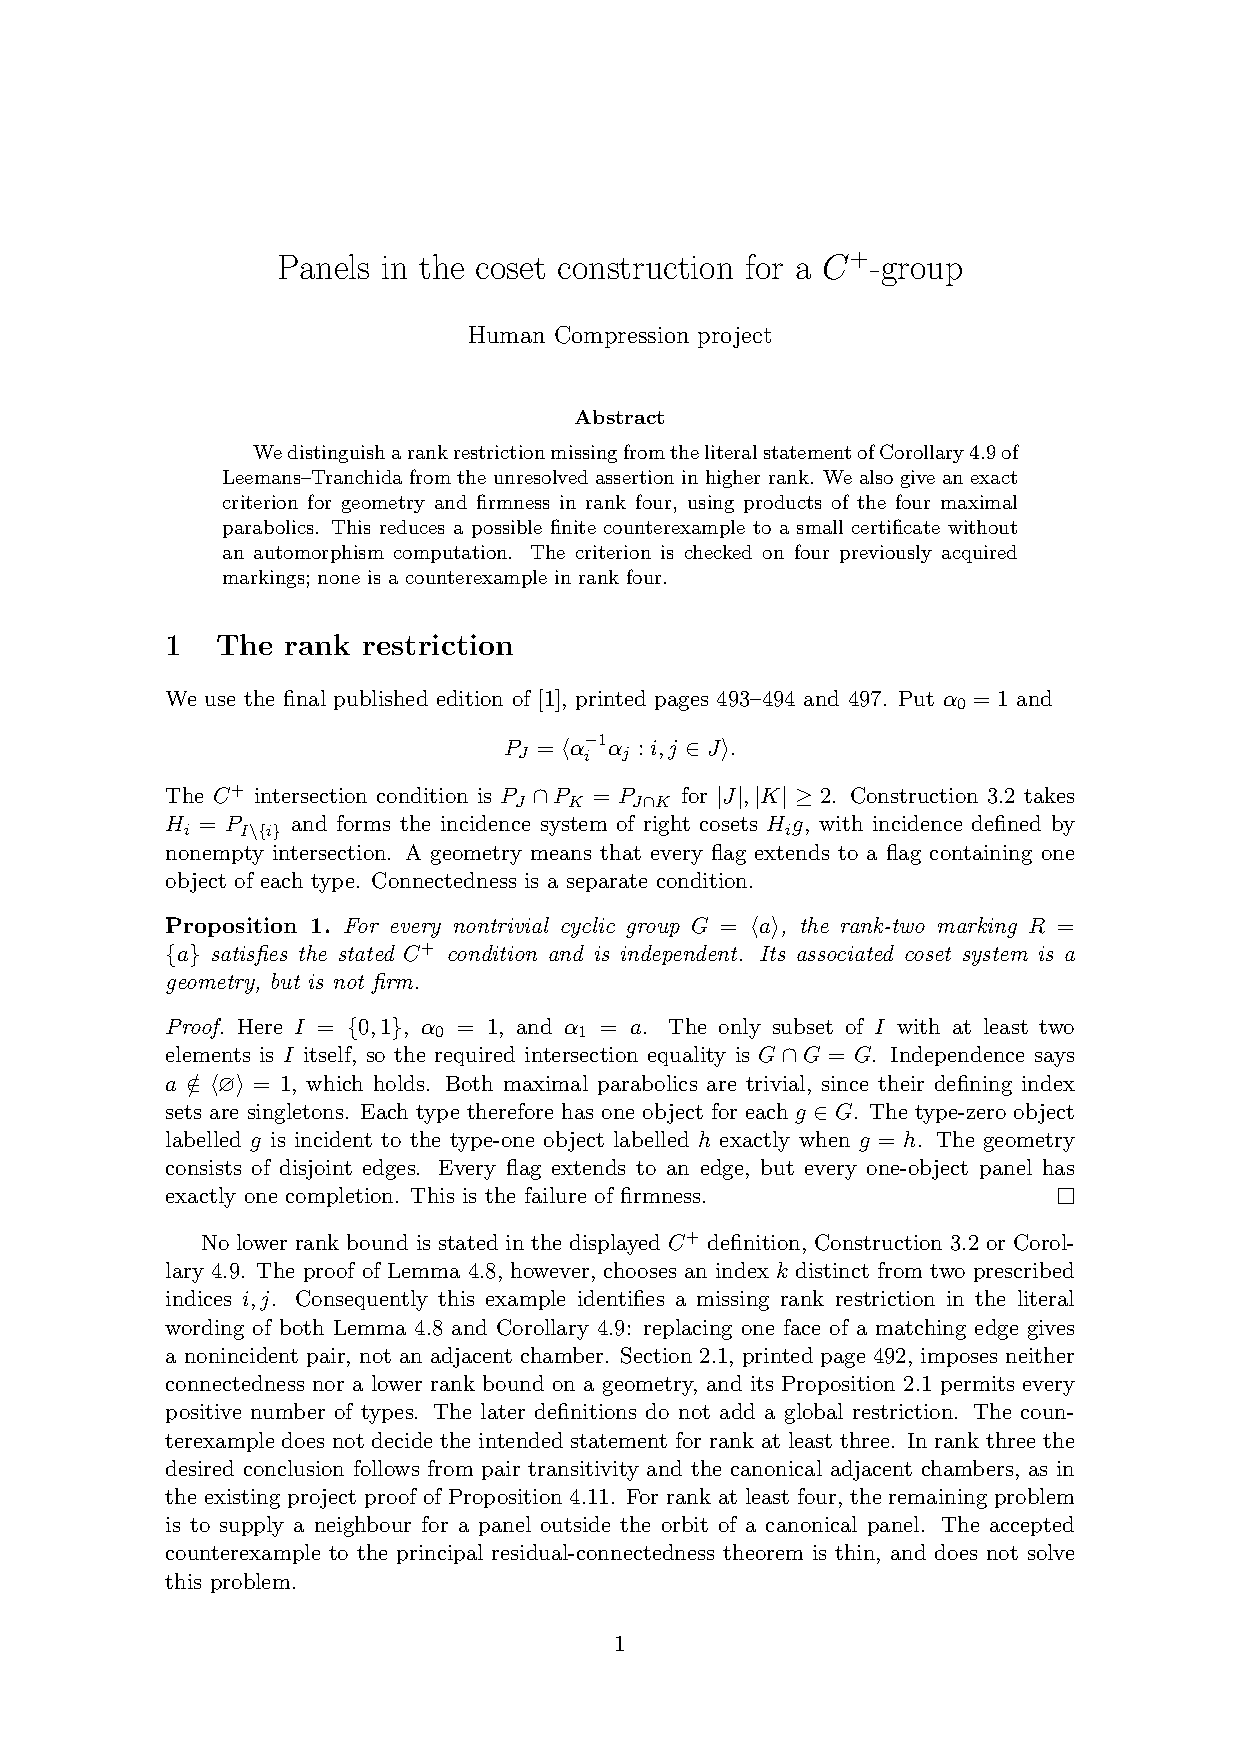
\includepdf[pages=-,pagecommand={},addtotoc={1,section,1,{Panels in the coset construction},panels}]{proofs/panels.pdf}
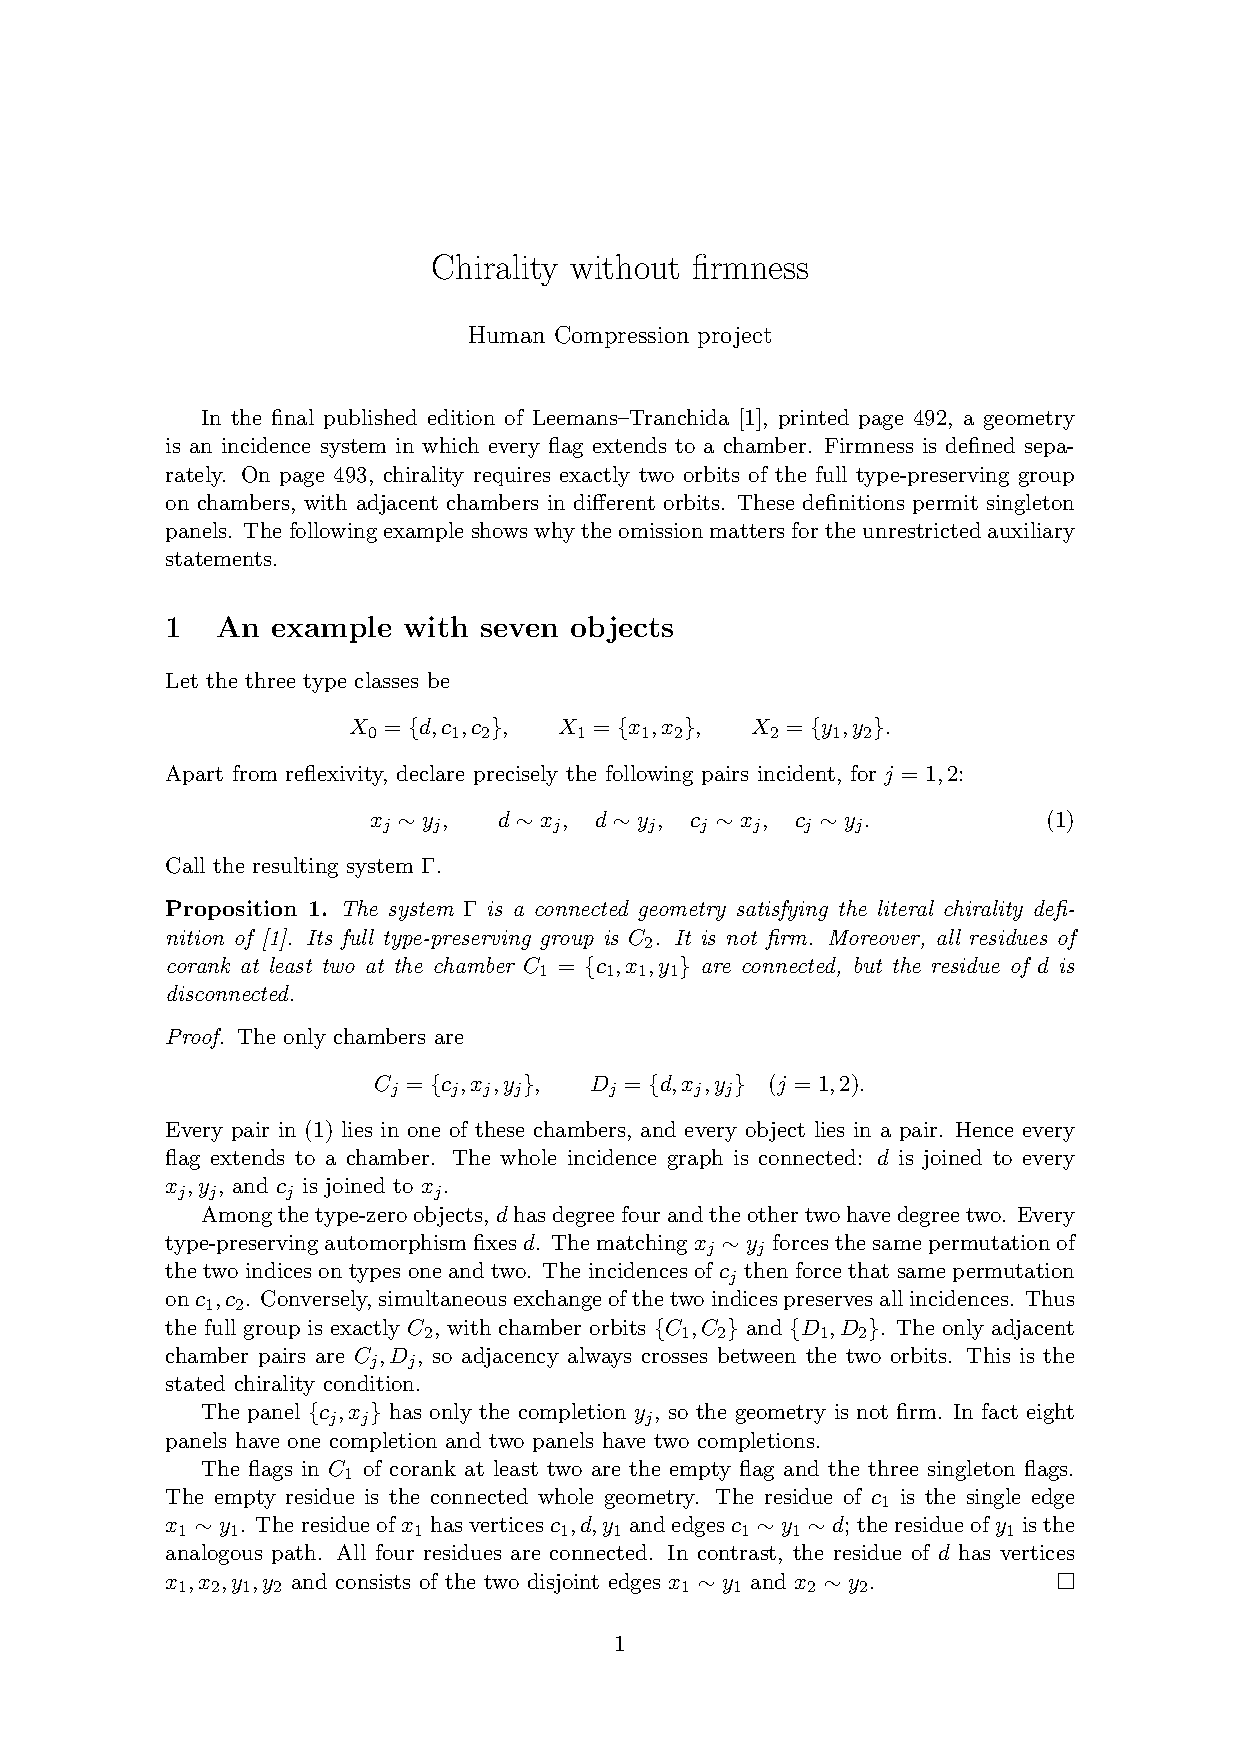
\includepdf[pages=-,pagecommand={},addtotoc={1,section,1,{Chirality without firmness},chirality}]{proofs/chirality.pdf}
\end{document}
